% Capítulo 2 - Nociones preliminares
\chapter[Nociones preliminares]{Nociones preliminares}
\label{chap:2}

En este capítulo introduciremos las definiciones y conceptos básicos con los que se trabajará durante el desarrollo de esta tesina. Se presentarán las \textit{redes de Petri} (\autoref{sec:2.petrinets}), la \textit{minería de procesos} (\autoref{sec:2.process mining}), \textit{Vectores Parikh} (\autoref{sec:2.parikh}),
\textit{Domínios numéricos abstractos} y su aplicación al desubrimiento de procesos (\autoref{sec:2.discovery}) así como los conceptos utilizados de \textit{logs} (\autoref{sec:2.logs}) e \textit{información negativa} (\autoref{sec:2.negative}).
\\

Por último, utilizando estos conceptos, plantearemos de manera concreta el problema a resolver en los capítulos siguientes (\autoref{chap:2.problem}).

\section{Redes de Petri}
\label{sec:2.petrinets}
Las \textbf{redes de Petri}, introducidas en el año 1962 por el matemático
Carl Adam Petri, consisten en una generalización de la teoría de automátas.
Nacidas de la necesida de de representar sistemas dinámicos con eventos concurrentes;
forman un lenguaje gráfico y matemático con una semántica formal.
Desde su creación, han sido utilizadas para, entre otros usos, para representación,
análisis, verificación y simulación de sistemas a eventos discretos con comportamiento dinámico\cite{Murata89}.

Una red de Petri esta formada por dos componentes, la red propiamente dicha y un conjunto
de \dquote{fichas} asignados a ciertos nodos de la misma.

La primera de estas componentes consiste en un grafo bipartito dirigido ponderado,
cuyos nodos se separan en los conjuntos dijuntos 
llamados lugares -\textit{places}- y transiciones -\textit{transitions}-.
Los arcos del grafo se dirigen tanto de los places a las transitions como viceversa.

En el momento de graficar una red de Petri, los places, por los general, se
representan mediante círculos y las transiciones mediante cajas o, simplemente, barras.

La segunda componente de una red de Petri consiste en la asignación
de un número entero de fichas o marcas a cada uno de los places, 
utilizado para simular el comportamiento dinámico y concurrente del sistema.
A la distribución de estas marcas sobre cada uno de los places, se la denomina
\textit{marking} y corresponde al estado en el cual se encuentra en cada momento el sistema.
La distribución inicial de estas fichas, por tanto, se conoce como \textit{marking inicial}.

Gráficamente, esta asignación se representa de manera distribuída, indicando dentro 
de cada place el número entero asignado por el marking, o bien, dibujando una 
cantidad de puntos igual a dicho número.
\\

Formalmente, una red de Petri es una 4-upla $(P,T,F,M_0)$ donde $P$ y $T$\footnotemark[1]
representan los conjuntos finitos y disjuntos de places y transitions respectívamente.
Por su parte, las transiciones ponderadas vienen dadas por \mbox{$F:(P \times T) \cup (T \times P)  \to \nat$}
y un marking $M$ viene dado por la función \mbox{$M:P \to \nat$}.
En particular, llamamos $M_0$ al estado inicial de la red, i.e. el marking inicial.

\footnotetext[1]{ En este trabajo, utilizamos el mismo símbolo $T$ para denotar el conjunto de transiciones -\textit{transitions}-
    de una red de Petri así como para el alfabeto de eventos de las trazas de un log.
    
    Esta colisión es intencionada ya que, en nuestro modelo, cada transición se corresponde biunivocamente
    con una actividad del log (solo consideramos la actividad completa y no el inicio/fin como en otros enfoques).
    Por esta razón, las transiciones silenciosas (aquellas donde su ejecución no puede ser observada)
    no son admitidas en la red y por la cual dos transiciones diferentes no pueden representar una misma acción.
}

Se denotan \textit{preset} y \textit{postset} de un place $p$ como $\preset{p}$ y $\postset{p}$ respectivamente,
los cuales se definen formalmente como: $\preset{p} =  \{t \in T ~|~ F(t,p) > 0 \}$
y $\postset{p} = \{t \in T ~|~ F(p,t) > 0 \}$.

Se le llama red de Petri \emph{pura} a una red que no posea ciclos de longitud uno, i.e.
$\forall p \in P:~ {\preset{p}} \mathrel{\cap} {\postset{p}} = \emptyset$.
En adelante, asumiremos que todas las redes de Petri con las que trabajamos son puras.
Esto es una consecuencia de utilizar la teoría de poliedros. Es importante destacar que esto no es una 
restricción importante ya que podemos, de manera sistemática, relajar un modelo no puro agregando
places ficticios y convertir cualquier lazo en un ciclo de longitud dos para obtener una red de Petri pura.
\\

Como notamos anteriormente, las redes de Petri se utilizan para representar sistemas 
dinámicos; este comportamiento dinámico está definido mediante las \emph{reglas de evolución}.

Decimos que una cierta transición $t \in T$ esta \emph{habilitada},
en un cierto marking $M$ si \mbox{$\forall p \in P:~ M(p) \ge F(p,t) $}.

Ejecutar una transición $t$ en un marking induce un nuevo marking $M'$
definido de manera incremental, como  \mbox{$M'(p) = M(p) - F(p,t) +  F(t,p)$},
para cualquier $p \in P$. A esta evolución la notamos \firing{M}{t}{M'}.

Una cierta secuencia de transiciones \mbox{$\sigma = t_1,t_2, t_3, \ldots, t_n$}
se dice ejecutable si existe una secuencia de markings \mbox{$\omega = M_1, M_2, \ldots, M_n$}
tal que ocurra la evolución
\firing {\firing {\firing {\firing {M_0} {t_1} {M_1}} {t_2} {M_2} } {t_3} {\cdots}} {t_n} {M_n}.

Dada una red de Petri $N$, llamamos $\Language(N)$ al lenguaje de la misma, i.e.
el conjunto de secuencias de transitions ejecutables sobre $N$.
Por su parte, al conjunto de markings alcanzable partiendo desde el marking inicial $M_0$,
llamado \emph{conjunto alcanzable} de $N$, lo notamos $\rs(N)$.

\begin{figure}[t]
  	\centering
    \begin{tikzpicture}

  \node[transition] (x) at (-.75,-1) {$x$};
  \node[transition] (y) at (.75,-1) {$y$};
  \node[tplace,label=above:$p_1$] (p1) at (0,0) {};
  \node[tplace,label=below:$p_0$] (p2) at (0,-2) {};
      
  \node[] (t) at (p1) {6};
  \node[] (t) at (p2) {1};
    
  \draw[style={->,>=triangle 45}] (p1) edge node[above left]{2} (x);
  \draw[style={->,>=triangle 45}] (x) to (p2);    
  \draw[style={->,>=triangle 45}] (p2) to (y);      
  \draw[style={->,>=triangle 45}] (y) edge node[above right]{3} (p1);
  
  \node[] (null) at (0,-3) {};
  
\end{tikzpicture}

    \caption{Una red de Petri (pura) con pesos no unitarios.}
    \label{fig:pn1}
\end{figure}

Consideremos ahora un place $p$ con
\mbox{$\preset{p}=\{x_1,\ldots,x_k\}$},
\mbox{$\postset{p}=\{y_1,\ldots,y_l\}$} y una función de transición 
$F$ igual a la función constante 1.
Siendo $M_0(p)$ la cantidad de tokens en el marking inicial 
para el place $p$, entonces, la siguiente ecuación
se satisface para cualquier secuencia de eventos $\sigma$

\bequationl{1place_cte}
M(p) = M_0(p) + \widehat\sigma(x_1)+\cdots +\widehat\sigma(x_k) -
\widehat\sigma(y_1)-\cdots -\widehat\sigma(y_l).
\eequation

La ecuación \eqref{eq:1place_cte}, puede generalizarse para permitir arcos
ponderados como

\bequationl{1place_wei}
M(p) = M_0(p) + \sum_{x_i \in \preset{p}}F(x_i,p)\cdot
\widehat\sigma(x_i) -
\sum_{y_i\in\postset{p}}F(p,y_i)\cdot\widehat\sigma(y_i).
\eequation

Si extendemos \eqref{eq:1place_wei} a todos los places de una red de Petri,
utilizando la notación matricial, tenemos

\bequationl{matrix_eq}
M = M_0 + A \cdot \widehat\sigma 
\eequation

donde $M$ y $M_0$ son vectores y $A$ representa la \emph{matriz de incidencia}
del grafo; $A$ posee $|P|$ filas y $|T|$ columnas y representa las conexiones 
existentes en la red.
A la ecuación \eqref{eq:matrix_eq}, se la llama \emph{ecuación de marking} de una red
de Petri~\cite{Murata89}.

Sea $\prs(N)$ el \emph{conjunto potencialmente alcanzable}
definido como el conjunto de soluciones de la siguiente ecuación,

\bequationl{matrix_ineq}
    M = M_0 + A \cdot \widehat\sigma \geq 0
\eequation

Utilizando la ecuación \eqref{eq:matrix_ineq} resulta simple definir el concepto
de complejidad de una red de Petri definida. El mismo consiste en la suma
de los valores absolutos de todos los coeficientes de la matriz $A$ con la suma
de los valores absolutos del vector de $M_0$.

A continuacion, a modo de ejemplo, construímos la ecuación \eqref{eq:matrix_ineq} de
la red de Petri de la ~\autoref{fig:pn1}, la cual es

\bequation
 \left[\begin{array}{c} 1 \\ 6 \end{array} \right] +
\left[\begin{array}{rr} 1 & -1 \\ -2 & 3 \end{array} \right]
\cdot
\left[\begin{array}{c} \widehat\sigma(x) \\ \widehat\sigma(y) \end{array}
\right]
\geq \left[\begin{array}{c} 0 \\ 0 \end{array} \right]
\eequation

Es importante ver que todo marking alcanzable de una red de Petri
satisface \eqref{eq:matrix_ineq}, sin embargo, lo opuesto no siempre es cierto.
En general, pueden existir markings no alcanzables para
los cuales \eqref{eq:matrix_ineq} se satisface, i.e. $\rs(N) \subseteq \prs(N)$~\cite{SilvaTC96}.

\section{Minería de procesos} 
\label{sec:2.process mining}

\subsection{Logs} 
\label{sec:2.logs}

La minería de procesos tiene su punto inicial en la recopilación de una serie de \textit{log de eventos}. 
Un evento efiere a una actividad, observable o no, de un sistema $\sys$ y
una traza de enventos -o simplemente traza- se define como una secuencia
ordenada de estos eventos, por lo general, generadas de manera automática.
Un log de eventos -o simplemente \textit{log}- por su parte, corresponde a un
conjunt de trazas. Un log corresponde a una instancia única de la ejecución de $\sys$,
llamada, instancia de proceso o caso y, durante la minería de procesos,
suelen utilizarse varíos casos sobre un mismo proceso~\cite{Aalst2004}.

Un log posee los siguientes elementos constitutivos fundamentales: un conjunto de actividades,
un cierto orden temporal en el cual ocurren y un caso o instancia de proceso que agrupe dichas actividades.
Sin embargo, un log pueden contener, además, datos adicionales que, aunque no sean fundamentales, pueden
ayudar a la minería de procesos otorgándole mayor nivel de detalle y claridad.

La tabla \autoref{tab:log_ex} muestra un ejemplo parcial de un conjunto de logs con información adicional (i.e. medio, actividad, nivel) que permite un entendimiento mayor del devenir del proceso,

\begin{table}[t]
\tiny

\def\sep{\hspace{10pt}}
\begin{tabular}{r   c   l   l   r   c   c}
  \tiny \#Caso
& \tiny Timestamp
& \tiny Medio
& \tiny Tipo
& \tiny Urgencia
& \tiny Usr
& \tiny Grupo
\\
\midrule
 970 & 2015-12-31 23:55:12 & Teléfono & Aviso & 0 & Andrés & Nivel 1\newrow
 970 & 2015-12-31 23:56:22 & Mail & Reclamo & 0 & Andrés & Nivel 1\newrow
 970 & 2016-01-01 00:05:11 & Teléfono & Reclamo & 1 & Andrés & Nivel 1\newrow
 971 & 2016-01-01 00:30:44 & Mail & Abierto & 2 & Gonzalo & Nivel 1\newrow
 971 & 2016-01-01 00:30:44 & Mail & Resuelto & 2 & Gonzalo & Nivel 1\newrow
 970 & 2016-01-01 00:30:44 & Teléfono & Derivado & 0 & Andrés & Nivel 2\newrow
 312 & 2016-01-01 15:30:01 & Mail & En progr. & 3 & Gonzalo & Nivel 3\newrow
 42 & 2016-05-04 00:00:01 & Mail & Resuelto & 10 & Lucio & Nivel x\newrow
 42 & 2016-05-04 00:00:01 & Mail & Resuelto & 10 & Lucio & Nivel x\newrow
 $\vdots$ & $\vdots$ & $\vdots$ & $\vdots$ & $\vdots$ & $\vdots$ & $\vdots$ \newrow
\end{tabular}
\vspace{0pt}
\caption{\tiny Un ejemplo artificial de un log de eventos con información adicional.}
\label{tab:log_ex}
\end{table} 


Formalmente, dado un alfabeto $T$\footnote{Ver nota previa referente a la colisión de nombres} representando
al conjunto de posibles eventos, un log se define como un conjunto $\pmlog \in \mathcal{P}(\eventstar)$\footnote{
Los logs pueden ser definidos de manera más general como multiconjuntos donde algunos comportamientos
pueden ser observados múltiples veces. No consideramos este enfoque ya que no consideramos 
la frecuencia de cada traza; las redes solo contemplan la presencia o ausencia de un cierto comportamiento.}. 


Los elementos del log \pmlog, llamados \textit{trazas}, son secuencias de eventos de $T$,
i.e. $\sigma \in \eventstar$. 
Por abuso de notación, se utiliza $\sigma \in \sys$, para indicar que existe una ejecución del sistema $\sys$
en la que s presentan los eventos de $\sigma$ de manera ininterrumpida y ordenada.

Dados un numero natural $1 \leq k \leq n$ y una traza $\sigma=\sigma_1\cdot\sigma_2\cdot\ldots\cdot\sigma_n$, a la traza
$\sigma_{k+1},\sigma_{k+2},\dots,\sigma_n$ se la llama sufijo de $\sigma$ y a la traza
$\sigma_1,\sigma_2,\dots,\sigma_k$ se la llama prefijo de $\sigma$.

%Abusando de notación,  si una cierta traza $\sigma'$ es el prefijo de alguna traza de $\pmlog$, se dice que 
%$\sigma' \in \pmlog$ .

\subsection{Minería de procesos} 
\label{sec:2.process mining subsection}

La \textit{minería de procesos} -\textit{PM} por sus siglas en inglés \textit{Process Mining}-
es una disciplina de investigación que intenta describir, analizar y mejorar cualquier
tipo de proceso informatizado. Se puede dividir la minería de procesos en tres grandes técnicas: descubrimiento (automatizado)
de procesos (i.e. extraer un modelo del proceso a partir de un log), validación de procesos (i.e. controlar posibles fallas 
al comparar un modelo con un log) y mejora de modelos (i.e. corregir un cierto modelo basado en la información extraída de los logs)~\cite{Aalst2004}~\cite{AalstBook}~\cite{FahlandA15}.
En ~\autoref{fig:pmcycle} se muestra como se relacionan los diferentes tipos de PM entr sí, con los logs de un sistema
y con otros modelos, en búsqueda de un modelo de los procesos de un cierto sitema

\begin{figure}[t]
  	\centering
    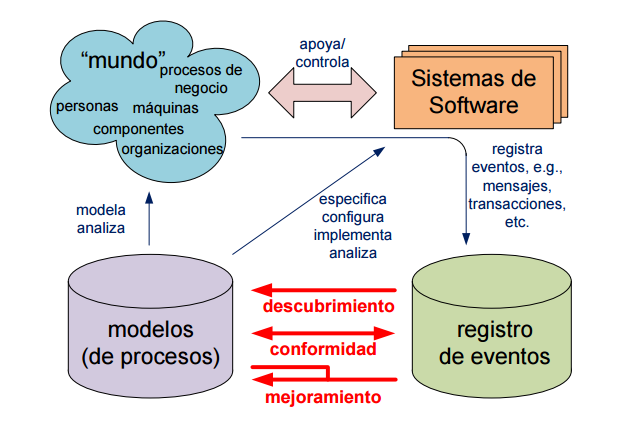
\includegraphics[scale=0.5]{img/pmcycle.png}\\
    \caption{Interacción de los diferentes tipos de PM.}
    \label{fig:pmcycle}
\end{figure}

Al relacionar el comportamiento de $\pmlog$, $\Language(N)$ y $\sys$, se definen nuevos conceptos~\cite{BuijsDA14}: modelo \emph{incompleto},
modelo \emph{adecuado} -\textit{fitting}-, modelo \emph{preciso}, modelo \emph{generalizador} de un log y \emph{simpleza} de un modelo.

\begin{itemize}
  \item $\pmlog$ se dice incompleto con respecto a un sistema $\sys$ si existen comportamientos
        de $\sys$ no representados en $\pmlog$.
        i.e. ${\sys} \setminus \pmlog \ne \emptyset$.
  \item $N$ se dice fitting con respecto a un log $\pmlog$ si el modelo captura el comportamiento 
        de los eventos en $\pmlog$, indica cuanto del comportamiento observado acepta $N$. 
        i.e. $\pmlog \subseteq \Language(N)$.
  \item $N$ se dice preciso con respecto a un log $\pmlog$ si $N$ no admite ejecuciones que no hayan
        sido observados en $\pmlog$ .
        i.e. $\Language(N) \setminus \pmlog = \emptyset$.
  \item $N$ se dice una generalización de un log $\pmlog$ sobre un sistema $\sys$ si $N$
        no es totalmente específico, restringiendose al comportamiento observado en $\pmlog$.
        i.e. $({\sys} \setminus \pmlog) \cap \Language(N) \neq \emptyset$.
  \item $N$ se dice simple cuando posee la menor complejidad posible y representa $\Language(N)$,
        i.e. la aplicación de la famosa \emph{navaja de Ocamm}.
        Es ampliamente aceptado que el tamaño de un modelo de procesos constituye el indicador más importante
        sobre la simplicidad del mismo~\cite{AalstBook}~\cite{Aalst2012}~\cite{LeonRCHH15}~\cite{CarmonaC14}.
\end{itemize}

El primero de los enfoques de la minería de procesos, el descubrimiento de procesos, busca extraer un modelo $N$
(e.g. diagrama UML, BPMN, red de Petri) a partir de un log $\pmlog$ con el objeto de modelar
el proceso subyacente en un cierto sistema, $\sys$. 

La validación de procesos, por su parte, comprende analizar la calidad de un cierto modelo,
posiblemente obtenido mediante las técnicas de descubrimiento del punto anterior. En este punto, 
son necesarios, por lo menos, un modelo $N$ y un log $\pmlog$ y consiste en medir la calidad 
de $N$ en reproducir los comportamientos observados en $\pmlog$. Para medir la calidad de $N$ se 
utilizan los conceptos ut supra definidos:
Se busca un modelo \emph{fitting}, \emph{preciso}, \emph{general} y \emph{simple}.

Por último, la mejora de modelos, se preocupa de extender y mejorar un modelo dado utilizando la información
del proceso real obtenida a partir de los logs. En este punto, se buscan detectar posibles dificultades en 
el modelo así como también reducir su complejidad. 

\section{Vectores Parikh} 
\label{sec:2.parikh}

Dado una traza $\sigma=\sigma_1\cdot\sigma_2\cdot\ldots\cdot\sigma_n$, sobre un alfabeto
$T={t_1,t_2,\dots,t_n}$, se utiliza $|\sigma|_{t_i}$ para representar la
cantidad de ocurrencias de $t_i$ en $\sigma$.
Luego, el \emph{vector Parikh} de una secuencia de eventos se define como

\begin{definition}
    \label{def:pv}
    (Vector Parikh). Sea $T=\{t_1,\ldots,t_n\}$ un alfabeto de eventos,
    el vector Parikh de una secuencia de eventos sobre $T$ se define como
    la función

    \bequation
        \begin{array}{lll}
            \widehat{\ }:& T^*&\rightarrow \nat^n\\
            %\;&\sigma &\mapsto \widehat{\sigma}=(|\sigma|_{t_1},\dots, |\sigma|_{t_n} )\\
            \widehat{\sigma}&=&(|\sigma|_{t_1},\dots, |\sigma|_{t_n} )
        \end{array}.
    \eequation
Además, por simplicidad, se nota cada $|\sigma|_{t_i}$ como $\widehat\sigma(t_i)$.
\end{definition}

\begin{definition}
    \label{def:pv_log}
    (Vectores Parikh de un log). Dado un log $\pmlog$, el connjunto de
    vectores Parikh de $\pmlog$ se define como

    \bequation
        \parikh{\pmlog}=\{ \widehat\sigma ~|~ \sigma \in \pmlog \}.
    \eequation

\end{definition}

E.g. dadas las trazas  $\sigma_1=t_1 \cdot t_2 \cdot t_1 \cdot t_2 \cdot t_1 \cdot t_1 \cdot t_3$
y $\sigma_2=t_4 \cdot t_4$ sobre el alfabeto $T=\{t_1,t_2,t_3,t_4\}$,
se tiene que los vectores Parikh de cada traza son: $\widehat{\sigma_1} = (4,1,1,0)$ y
$\widehat{\sigma_2} = (0,0,0,2)$ y si se toma \mbox{$\pmlog =\{\sigma_1,\sigma_2\}$}
se tiene que $\parikh{\pmlog}=\{ (0,0,0,2),(4,1,1,0) \}$.

Dado que los vectores Parikh no consideran el ordern de los eventos, la función \mbox{$\widehat{\ }$} no 
es una función inyectiva, i.e. dos trazas diferentes pueden poseer la misma representación como Parickh
vector.
%However since we transform every prefix of a trace into a point,
%there is no loss in expressivity:
%traces $a \cdot b$
%and $b \cdot a$ generate the vector $(1,1)$,
%however the former also generates $(1,0)$ since this is the Parikh vector of its prefix $a$,
% but this vector is not generated by $b \cdot a$.

\section{Información negativa} 
\label{sec:2.negative}

Existen diferentes términos para el término \textit{información negativa}. Por ejemplo, en aprendizaje automático,
el término hace referencia a un comportamiento que posee una etiqueta negativa, e.g. para un grupo
de estudiantes de un curso, la información positiva corresponden a aquellos estudiantes que aprueban el curso
y la información negativa, aquellos estudiantes que reprueban el curso. 

En el campo de la minería de procesos, por lo general, la noción utilizada de información negativa es diferente;
una traza negativa corresponde a un comportamiento prohibido, una secuencia de eventos que se desea 
evitar durante la ejecución del sistema y como tal no debe ser aceptado en el modelo.

\begin{definition}
    \label{def:neg}
    (Trazas negativas) Una cierta traza $\sigma=\sigma_1\cdot\sigma_2\cdot\ldots\cdot\sigma_n$ es
    una traza negativa (o prohibida) del sistema $\sys$ si $\exists k \in \nat, k \lneq n$ tal que
    el prefijo $\sigma'=\sigma_1\sigma_1\cdot\sigma_2\cdot\ldots\cdot\sigma_k \in \sys$ pero $\sigma \notin \sys$
\end{definition}

Debido al hecho de que los logs de eventos existentes en la vida real rara vez contienen información negativa, 
en este trabajo se utilizan métodos alternativos automáticos de obtener dicha información. En ~\cite{Goedertier2009} 
y ~\cite{BrouckeWVB14} se presentan métodos metodos eficientes de inducir la llamada \textit{información negativa artificial},
basada en la informaciñon positiva. 

En el ámbito de la minería de procesos, no es el utilizado en estra trabajo el único
concepto admisible de trazas negativas. 
%En \cite{Goedertier2009,BrouckeWVB14}  el concepto utilizado es de una traza positiva
%a la cual se las concatena con un único evento negativo.
%Corresponde al caso particular en que para todas las trazas negativas,
%según la definición \autoref{def:neg}, $|\sigma'|=k=n-1$. 

Se utiliza la definición \autoref{def:neg}, una versión más general 
a la utilizda en \cite{Goedertier2009,BrouckeWVB14}. Se utilizan sufijos
automaticos sobre las trazas negativas obtenidas del algoritmo 
descrito en ~\cite{BrouckeWVB14}.
Esta generalización responde al hecho  de que las trazas negativas 
son tranformadas en puntos negativos y luego estos son utilizados
para restringir el proceso de expansión y/o rotación en pos de mejorar el modelo.
Las trazas de la forma utilizada en \cite{Goedertier2009,BrouckeWVB14} generan
puntos negativos que se encuentran muy cercanos al poliedro generado, reduciendo la aplicabilidad del 
método presentado en el trabajo.

\section{Domínios númericos abstractos y descubrimiento de procesos} 
\label{sec:2.discovery}

\subsection{Poliedros convexos y látices enteras} 
\label{sec:2.discovery polyhedra}

Un \textit{semiespacio} es cada
una de las porciones en las que queda dividido un espacio $n$-dimensional por un hiperplano $(n-1)$-dimensional. Un semiespacio
puede ser descripto mediante un incuación lineal de la forma $a_1x_1 + a_2x_2 + \cdots + a_nx_n \geq b$.

Un poliedro convexo $n$-dimensional es un conjunto convexo de puntos en $\mathbb{R}^n$. Existen 
dos maneras de representar un poliedro convexo, la $V$-representación y la $H$-representación~\cite{Rockafellar70}.
En este trabajo, se utiliza la segunda, la cual representa un poliedro convexo $\ph$ 
como la intersección de un conjunto de $k$ hiperespacios,

\bequationl{convex_poly}
    \ph = \{ x \in \mathbb{R}^n ~|~ A\cdot x + b \geq 0\}
\eequation
donde  \mbox{$A \in \mathbb{R}^{k \times n}$} y
\mbox{$b\in\mathbb{R}^{k}$}.

Los siguientes resultados son importantes para el resto del trabajo~\cite{CarmonaC14},

\begin{theorem}
\label{theo:orig_in_b_pos}
    Sea $\ph$ un poliedro convexo definido como la intersección de un conjunto
    finito de semiespacios siguiendo \eqref{eq:convex_poly}. $\ph$ contiene el 
    origen \mbox{$z=(0,\ldots,0)$} sí y solo sí, $b \geq 0$
\end{theorem}

\begin{proof}
    Si el orgien pertene a $\ph$, entonces $b$ debe tener todas sus componentes positivas,
    en caso contrario una de las inecuaciones no se cumpliría al evaluar el origen.
    Por otro lado, si $b \geq 0$, entonces el origen satisface todas las inecuaciones.
\end{proof}

En adelante, cuano se habla simplemente poliedro se hace referencia a un poliedro convexo,
excepto que se indique lo contrario.
%Since we will use the convex polyhedron of the Parikh representation of a log we restrict to the integer points inside it. 

Se denomina látice entera, y se nota $Z^n$, a una látice en el espacio Euclediano $\mathbb{R}^n$
cuyos puntos son $n$-uplas de enteros. 

Dado un poliedro convexo $\ph$, el conjunto de puntos enteros dentro de $\ph$
forman una látice entera, denominada $Z$-poliedro de $\ph$.
% Cambió de idioma y se transvistió...

\subsection{Descubrimiento de procesos} 
\label{sec:2.discovery discovery}

El objetivo del \textit{descubrimiento de procesos} es encontrar un 
modelo $N$ (e.g. una red de petri) que represente, el comportamiento 
observado en un cierto log $\pmlog$.

En ~\cite{CarmonaC14} se presentan diferentes técnicas 
para el descubrimiento de redes de Petri a partir del 
conjunto de vectores Parikh de un log $\pmlog$.

Se utliza el conjunto $\parikh{\pmlog}$ para encontrar
una $A$ y marking inicial $M_0$ según \eqref{eq:matrix_eq};
de esta manera la red de Petri que se obtiene resulta 
una buena aproximación del proceso que genera el log $\pmlog$.

Dada una red de Petri $N$, comparando las expresiones \eqref{eq:matrix_eq}
y \eqref{eq:convex_poly}, se puede observar que $\prs(N)$ se corresponde con
un $Z$-poliedro de un poliedro convexo que posee dos propiedades:
\mbox{$A \in \mathbb{Z}^{|P|\times|T|}$} y \mbox{$M_0 \in \mathbb{N}^{|P|}$}.
Estas propiedades, se garantizan debido a que el marking inicial no es negativo 
y sólo markings con valores enteros positivos son alcanzables.


La látice entera n-dimensional $\mathbb{Z}^n$ es la látice de las $n$-uplas
de enteros que representan a los elementos de $\parikh{\pmlog}$. Así, un log 
puede representarse como un conjunto de caminatas en $\mathbb{N}^n$. Cada paso en
una caminata se mueve de un punto de la látice a otro aumentando únicamente uno de
los componentes de la $n$-upla en una unidad.

En \autoref{fig:simp}, se ilustra ver la correspondencia entre un log y una red
de Petri. La figura a la izquierda.

\begin{figure}
  \centering
  \subbottom[\label{sfig:simp.1}]{%
    \scaledinput{0.37}{img/ineq}}
  \hfill
  \subbottom[\label{sfig:simp.2}]{%
    \scaledinput{0.9}{img/ineq_net1}}
  \hfill
  \subbottom[\label{sfig:simp.3}]{%
    \scaledinput{0.9}{img/ineq_net2}}
  \caption{Caminatas en la látice entera y red de Petri.}
  \label{fig:simp}
\end{figure}


En ~\autoref{sfig:simp.1} representa tres caminatas en un espacio bidimensional.
Las áreas en grís claro representan un poliedro que contiene todos los puntos
visitados por las tres caminatas. Dicho poliedro, puede representarse como 
la intersección de dos semiespacios en $\mathbb{R}^2$

\bequation
    \begin{array}{lllllll}
        1&+&\widehat\sigma(x)&-&\widehat\sigma(y)&\geq&0\\
        6&-&2\cdot\widehat\sigma(x)&+&3\cdot\widehat\sigma(y)&\geq&0
    \end{array}.
\eequation

El poliedro puede ser representado también, de la forma de la ecuación \eqref{eq:matrix_ineq} 
obteniendo así la interpretación de la ecuación de marking para la red de Petri en ~\autoref{sfig:simp.2}.
Cada semiespacio del poliedro, i.e. cada fila de la matriz, está representado por un place de la red.
El conjunto de vectores Parikh generados por esta red corresponden al $Z$-poliedro del poliedro 
representado en ~\autoref{sfig:simp.1}.

En resumen, dada un log $\pmlog$, podemos aplicer las técnicas introducidas en ~\cite{CarmonaC14}
al conjunto $\parikh{\pmlog}$ para obtener un poliedro que pueda luego ser transformado en 
una red de Petri siguiendo un razonamiento análogo al enunciado.

\begin{remark}
    Al haber introducido ya la relación existente entre semiespacios y places de una red, 
    se explica por qué el método utilizado se limita a redes de Petri puras. 

    Si se considera un place $p$ el cual se encuentra tanto en el preset como en el postset
    de una transición $t$ y se asume una relación de flujo unitario, la variable que representa
    a $t$ en el semiespacio correspondite a $p$ no podrá capturar el hecho de que la transición
    es producida ($t$ con un coeficiente positivo) y consumida ($t$ con un coeficiente negativo) 
    al mismo tiempo. Esto se debe a que los coeficientes (i.e. $+1,-1$) se cancelan mutuamente.

    Por esto, el enfoque utlizado, solo considerará redes de Petri puras.
\end{remark}

\section{Enunciado del problema} 
\label{sec:2.problem}

Dado un log $\pmlogp$ y un conjunto de trazas negativas $\pmlogn$ el objetivo de las técnicas utilizadas 
en el desarrollo de la tesina es derivar un modelo $N$ con las siguientes caraterísticas\\

\begin{itemize}
 \item $N$ es una red de Petri pura ponderada;
 \item $\forall \sigmap \in \pmlogp:~ \sigmap \in \Language(N)$;
 \item $\forall \sigman \in \pmlogn:~ \sigman \notin \Language(N)$;
 \item $N$ minimiza su complejidad.\\
\end{itemize}

Los primers tres items son triviales ya que son garantizados por la metodología utilizada
para generar la red.

\section{Resumen del capítulo}
\label{sec:2.resumen}
En este capítulo se hizo una introducción a diferentes temas fundamentales para la comprensión y el desarrollo de este trabajo. 
Se presentaron conceptos cruciales como \textit{redes de Petri}, \textit{minería de procesos},
\textit{poliedros convexos} y \textit{látices enteras}; se dieron definiciones como la de \textit{Vector Parikh} 
y \textit{vectores Parikh de un log} y se describireron ciertas nociones 
utilizadas como las de \textit{logs}, \textit{información negativa} 
o el concepto  entendido por complejidade de una red de Petri.

En particular, se ejemplificó la relación que existe entre ciertas redes de Petri con una látice entera y 
como utilizar esta relación para generar un primer modelo de un sistema a partir de un cierto log.

Por último, utilizando estos conceptos, se presentó una definición formal del problema a tratar en el desarrollo
 de la presente tesina. 
